\documentclass[conference]{IEEEtran}

\usepackage[utf8]{inputenc}
\usepackage[T1]{fontenc}
\usepackage{graphicx}
\usepackage{listings}
\usepackage{xcolor}
\usepackage{booktabs}
\usepackage{enumitem}
\usepackage{caption}
\usepackage{subcaption}
\usepackage{float}
\usepackage[colorlinks=true,linkcolor=blue,citecolor=blue,urlcolor=blue]{hyperref}

% Code listing styles
\definecolor{codebg}{RGB}{248,249,250}
\definecolor{codekw}{RGB}{0,100,180}
\definecolor{codestring}{RGB}{180,0,0}
\definecolor{codecomment}{RGB}{100,120,100}

\lstdefinestyle{xmlstyle}{
  backgroundcolor=\color{codebg},
  basicstyle=\ttfamily\footnotesize,
  keywordstyle=\color{codekw}\bfseries,
  stringstyle=\color{codestring},
  commentstyle=\color{codecomment}\itshape,
  breakatwhitespace=false,
  breaklines=true,
  captionpos=b,
  keepspaces=true,
  showstringspaces=false,
  frame=single,
  rulecolor=\color{gray!40},
  xleftmargin=0.5em,
  xrightmargin=0.5em,
  language=XML
}

\lstdefinestyle{pythonstyle}{
  backgroundcolor=\color{codebg},
  basicstyle=\ttfamily\footnotesize,
  keywordstyle=\color{codekw}\bfseries,
  stringstyle=\color{codestring},
  commentstyle=\color{codecomment}\itshape,
  breaklines=true,
  frame=single,
  rulecolor=\color{gray!40},
  xleftmargin=0.5em,
  language=Python
}

\lstdefinestyle{bashstyle}{
  backgroundcolor=\color{codebg},
  basicstyle=\ttfamily\footnotesize,
  breaklines=true,
  frame=single,
  rulecolor=\color{gray!40},
  xleftmargin=0.5em
}

% ─────────────────────────────────────────────────────────────
\begin{document}

\title{Threat Detection, Monitoring and Prevention\\in a Smart City Service-Oriented Architecture}

\author{%
  \IEEEauthorblockN{Eduardo Lopes}
  \IEEEauthorblockA{%
    Security in Large-Scale Systems\\
    Master's in Cybersecurity - DETI, University of Aveiro\\
    \today
  }
}

\maketitle

\begin{abstract}
A security monitoring and active-response platform was designed for a Smart City
Environmental Monitoring system built as a Service-Oriented Architecture across three
geographic zones. Four threat classes are addressed: HTTP flooding, distributed botnet
DDoS, a two-stage Advanced Persistent Threat via endpoint reconnaissance and honeypot
credential capture, and two email spam variants targeting the alert channel and the
SMTP transport layer. Detection relies on thirteen custom Wazuh rules. Automated
response is enacted through a threat-blocker service that applies \texttt{iptables}
DROP rules in the Docker bridge chain. Prometheus and Grafana provide real-time
observability across all threat classes. Seven attack surfaces are identified, of which
four are actively defended and three are documented as residual risks.
\end{abstract}

\section{Introduction}
\label{sec:introduction}

Modern cities increasingly deploy sensor-based platforms to monitor environmental
conditions (air quality, temperature, noise levels) and feed real-time data to operators
who must react to degraded conditions. As these platforms adopt Service-Oriented
Architectures (SOA) built on microservices, they inherit the security challenges of distributed
systems: an expanded attack surface, heterogeneous trust boundaries, and complex
inter-service communication that must be secured without introducing prohibitive latency.

This project presents the design, implementation, and evaluation of a threat detection
and prevention system for a Smart City Environmental Monitoring Platform built as a SOA.

\subsection{Scope}

The system addresses four threat classes, with two sub-variants of the spam threat:

\begin{enumerate}[leftmargin=*]
  \item \textbf{HTTP Flood (DoS):} volumetric single-source flood targeting the
        operator portal, aiming to blind city personnel before or during a physical event.
  \item \textbf{Advanced Persistent Threat (APT):} stealthy, multi-stage intrusion
        combining reconnaissance and targeted exploitation to gain unauthorised access
        to internal platform resources.
  \item \textbf{Alert Flood:} abuse of legitimate platform functionality to generate
        a high volume of automated notifications, degrading operator situational awareness.
  \item \textbf{Drug Content Spam:} unsolicited email containing illicit pharmaceutical
        content, targeting the platform's mail infrastructure as a delivery channel.
  \item \textbf{Botnet DDoS:} distributed volumetric attack orchestrated across multiple
        compromised nodes, overwhelming the target service through coordinated flooding.
\end{enumerate}

The APT and Alert Flood threats form a multi-stage attack chain: initial intrusion
enables subsequent service abuse, mirroring the lateral movement and impact phases of
real-world adversarial campaigns.

The remainder of this report is organised as follows. Section 2 reviews the relevant
state of the art. Section 3 describes the service architecture. Section 4 presents the
risk management analysis and mitigation strategies. Sections 5 through 9 detail the
detection and response approach for each threat class. Section 10 evaluates the overall
solution, its thresholds, and its scalability. Section 11 draws conclusions and outlines
future work.

\section{State of the Art}
\label{sec:stateoftheart}

\subsection{Service-Oriented Architectures and Security}

The decomposition of monolithic applications into microservices
increases operational flexibility but multiplies the attack surface: each service endpoint
becomes a potential entry point, inter-service calls transit a shared network that may be
partially compromised, and credentials or tokens that authenticate service-to-service
communication must be protected across many processes and containers.

\subsection{Monitoring Tools}

Prometheus is an open-source, pull-based metrics platform originally developed
at SoundCloud. Its time-series data model and flexible PromQL query
language make it well-suited to microservice observability. Grafana
provides dashboarding over Prometheus and other data sources. Commercial alternatives
such as Datadog and Zabbix offer similar functionality but introduce cost and vendor
dependency. Open-source tooling is preferred in this project to maintain transparency
over the detection pipeline.

\subsection{SIEM and Intrusion Detection}

Wazuh is an open-source SIEM derived from OSSEC. It ingests
log files, applies pattern-matching and frequency rules, and can trigger active responses
(shell scripts) on rule matches. It is the platform adopted in this project for
consistency with the course practicals. Commercial platforms such as Splunk provide
richer analytics but hide the underlying rule machinery. Falco targets
Kubernetes-specific syscall monitoring and does not apply to the Incus/Docker
deployment used here.

\subsection{DDoS Attacks and Mitigation}

DDoS attacks aim to exhaust the resources of a target service, rendering it unavailable
to legitimate users. Rate-based detection (triggering when a
source IP exceeds a request threshold within a time window) is a standard first-line
defence. Its limitation is that distributed floods (many source IPs) evade single-IP
thresholds, a limitation acknowledged in the evaluation.

\subsection{Advanced Persistent Threats}

APTs are characterised by stealth, persistence, and multi-stage execution.
The reconnaissance phase (endpoint enumeration, banner grabbing) precedes exploitation.
Honeypot-based detection (placing intentionally exposed
"decoy" endpoints that log all access) is a lightweight technique that generates high-fidelity
alerts: any access to a honeypot endpoint is inherently anomalous.

\subsection{Spam and Content Filtering}

Email spam remains a persistent threat vector, particularly in alert-driven operational
environments where operators are conditioned to act on incoming alerts. SpamAssassin applies a scoring model that combines header analysis, content
rules, and Bayesian classification. Its extensible rule system allows custom scoring for
domain-specific content (e.g., pharmaceutical keywords in a city monitoring context).
Application-layer alert flooding (using legitimate credentials to trigger high volumes of
internal alerts) is a distinct attack class that content filters cannot address alone and
requires circuit-breaker or rate-limiting logic at the application level.

\section{Service Architecture}
\label{sec:architecture}

\subsection{Domain and Motivation}

The platform models a Smart City Environmental Monitoring system serving a mid-sized
Portuguese city. The city is divided into three geographic zones: North (40.671°N, 8.627°W),
Centre (40.641°N, 8.654°W), and South (40.610°N, 8.681°W). Each zone has
IoT sensors reporting air quality (AQI), temperature (°C), and noise levels (dB). Each zone's sensors report
to a Zone Aggregator edge service, which computes per-interval statistics
(average, minimum, maximum) and sends a single batched payload to the central ingestion
service every 10 seconds. This aggregation pattern reduces upstream bandwidth by a factor
equal to the number of sensors per zone, limiting the volume of data
transmitted to the central platform.

\subsection{System Components}

\begin{figure*}[t]
  \centering
  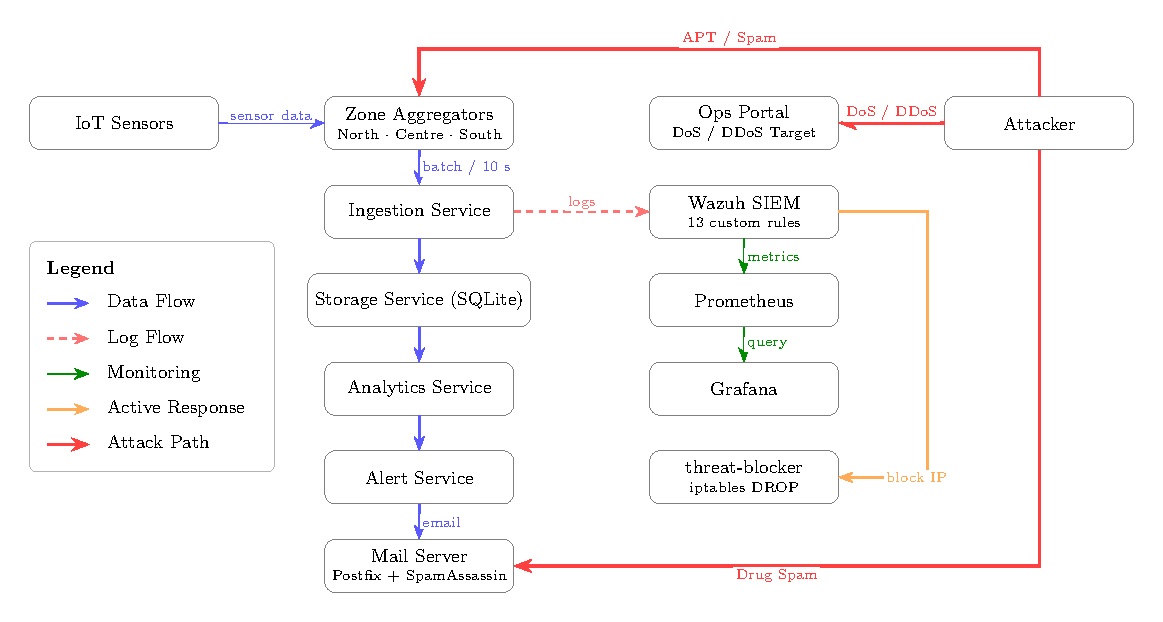
\includegraphics[width=\textwidth]{images/architecture.pdf}
  \caption{Smart City SOA infrastructure.}
  \label{fig:architecture}
\end{figure*}

Figure~\ref{fig:architecture} illustrates the full infrastructure, including data flows,
observability paths, and active response chain. Three zone aggregator services operate
on ports 5100, 5101, and 5102 for the
North, Centre, and South zones respectively. Each aggregator spawns three sensor
simulation threads, collects readings into a buffer, and forwards aggregated payloads
to the ingestion service. Access logs are written as structured JSON to a shared
volume mounted by Wazuh. Intentional honeypot endpoints (\texttt{/api/admin/config}
and \texttt{/api/admin/metrics}) are exposed to simulate a misconfigured debug
interface that leaks the \texttt{INTERNAL\_TOKEN} (the shared secret used to
authenticate inter-service calls).

The central platform comprises six services:

\begin{itemize}[leftmargin=*]
  \item \textbf{Service registry} (port 5050) - zone-aware service discovery with
        geographic metadata. Services register on startup and send heartbeats every 30 seconds.
  \item \textbf{Ingestion service} (port 5200) - receives zone payloads, validates
        data ranges, and forwards to storage.
  \item \textbf{Storage service} - SQLite-backed persistence of time-series readings.
  \item \textbf{Analytics service} - Aggregation queries and zone statistics.
  \item \textbf{Alert service} (port 5500) - monitors thresholds and sends email
        alerts when sensor readings exceed configured limits. A circuit breaker enforces
        a 5 minute cooldown after 12 consecutive emails, and Postfix applies a hard
        rate limit of 30 messages per minute.
  \item \textbf{Ops portal} (port 5600) - web dashboard for city operators and the
        primary target of DoS and DDoS attacks.
\end{itemize}

The mail server runs Postfix 3.6 with SpamAssassin content filtering on port 25.
A custom Python exporter exposes Prometheus metrics on port 9154 by tailing
Postfix logs.

The monitoring stack comprises four components: Prometheus (port 9090) scrapes all
services at a 15-second interval; Grafana (port 3000) provides the security
dashboard; the Wazuh exporter (port 9100) bridges Wazuh to Prometheus by tailing
\texttt{alerts.json} and polling the Wazuh REST API; and the threat-blocker service
(port 9200) receives block requests from Wazuh's active response script and applies
\texttt{iptables} DROP rules in the \texttt{DOCKER-USER} chain, with automatic
unblock after 300 seconds.

\subsection{Communication and Data Flow}

Inter-service calls are authenticated via a shared token distributed through the
\texttt{x-internal-token} HTTP header, generated at deploy time and distributed via
an environment file. All services write structured JSON access logs (including
timestamp, client IP, method, path, event type, and zone) to a shared Incus
bind-mount, which Wazuh ingests in real time.

\subsection{Security Mechanisms}

\begin{itemize}[leftmargin=*]
  \item \textbf{Internal token authentication:} as described above, all inter-service
        calls require the shared token. Requests that fail this check are logged as
        \texttt{auth\_failed} events, triggering Wazuh rules 100100 and 100101.
  \item \textbf{Honeypot endpoints:} \texttt{/api/admin/config} and
        \texttt{/api/admin/metrics} on zone aggregators log every access as a
        \texttt{HONEYPOT\_HIT} event. There is no legitimate caller for these paths.
  \item \textbf{404 logging:} a FastAPI exception handler logs all requests to unknown
        paths as \texttt{not\_found} events, enabling recon phase detection.
  \item \textbf{IP-level blocking:} \texttt{threat-blocker} writes DROP rules to
        \texttt{DOCKER-USER} rather than the \texttt{INPUT} chain, correctly intercepting
        traffic that is DNAT-forwarded by Docker before it reaches service processes.
\end{itemize}

\subsection{Infrastructure and Deployment Rationale}

The platform runs inside a Debian 13 VirtualBox VM (8 GB RAM, 6 CPUs). Available disk space on the host constrained all
components to this single VM, which already had Incus installed with a running Wazuh
instance. Two isolation layers are therefore used: Incus system containers for
host-level isolation, and Docker Compose inside one of those containers for the SOA
services.

Docker Compose was chosen as a second layer because the SOA comprises fourteen
interdependent services that require a shared internal network with stable DNS
resolution between them.

Log sharing between the two isolation layers is achieved through two host-level
bind-mounts: one exposes the Docker service logs to Wazuh for real-time ingestion,
and one exposes the Wazuh alert output to the Docker stack for the Wazuh exporter
to read.

\section{Risk Management and Mitigation}
\label{sec:monitoring}

\subsection{Attack Surfaces}

\begin{figure*}[t]
  \centering
  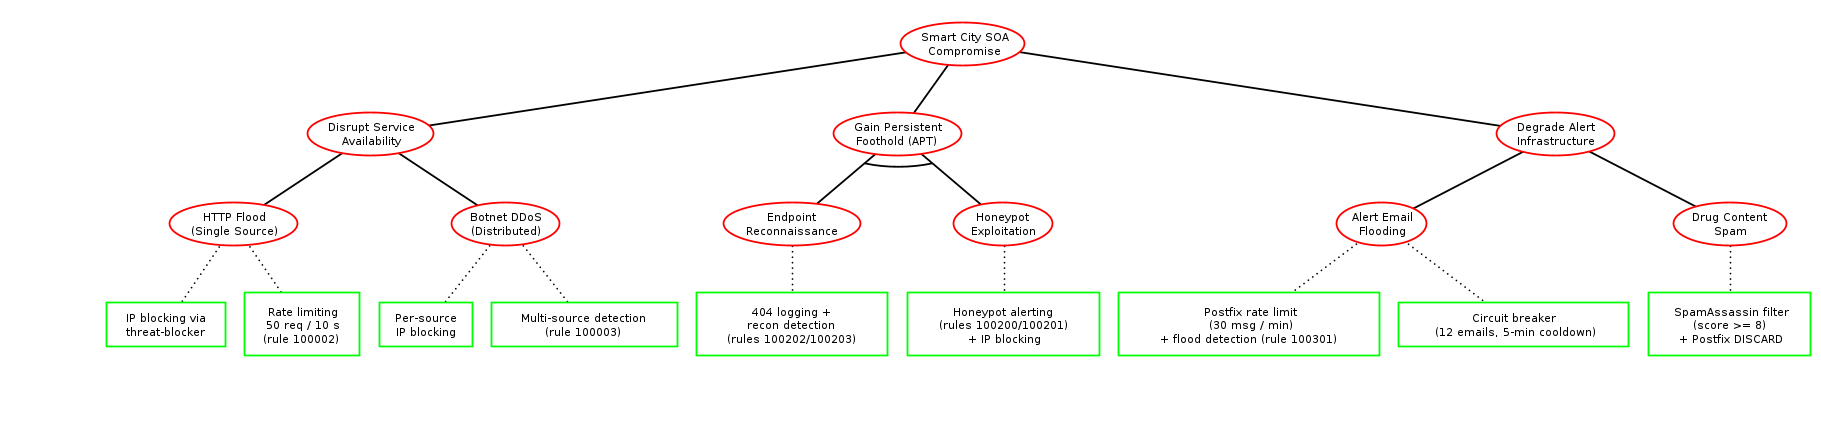
\includegraphics[width=\textwidth]{images/smart_city_attacktree}
  \caption{Attack-Defense Tree for the Smart City SOA. Red ovals represent attack nodes;
  green rectangles represent countermeasures.}
  \label{fig:attacktree}
\end{figure*}

Seven attack surfaces are identified in the Smart City SOA. Four are addressed by
the threat classes in Sections~5 through~9; three are recorded as residual risks
out of scope for the current implementation.

\begin{itemize}[leftmargin=*]
  \item \textbf{Public HTTP layer:} the ops portal accepts
        unauthenticated operator traffic and is reachable from outside the VM.
        A single high-rate source exploiting this interface constitutes a DoS
        threat. A coordinated set of sources acting in concert constitutes a
        DDoS threat. Neither attack requires application-level knowledge.
  \item \textbf{Inter-service API layer:} service-to-service calls are
        authenticated via the \texttt{x-internal-token} header, but that token
        is reachable through the honeypot endpoints on zone aggregators. A token
        obtained through endpoint enumeration enables impersonation of any
        internal service. This is a multi-stage surface, corresponding to the
        APT threat class. The conjunctive structure of that branch in
        Figure~\ref{fig:attacktree} reflects the two-phase dependency.
  \item \textbf{Mail delivery path:} two independent surfaces exist on the mail
        channel. The alert service generates outbound notifications whose volume
        is bounded only by a circuit breaker, exposing the system to alert
        flooding. The Postfix relay on port 25 accepts inbound mail without
        content filtering at the transport layer, exposing the system to
        drug-content spam. Each maps to a distinct threat class.
  \item \textbf{Observability and logging path:} Wazuh ingests logs from a
        shared Incus bind-mount. A compromised container writing malformed JSON
        to that volume could disrupt rule processing. This surface is not
        addressed in the current implementation and is recorded as a residual
        risk.
  \item \textbf{Zone aggregator sensor endpoints:} zone aggregators are
        internal edge services, but ports 5100-5102 are externally mapped in
        the lab deployment to allow the PoC scripts to reach the honeypot
        endpoints. This exposes the sensor ingestion endpoints directly: an
        attacker could POST fabricated readings, corrupting stored data and
        triggering false threshold alerts without touching the honeypot. In a
        production deployment, zone aggregators should reside on an internal
        network segment reachable only by the ingestion and analytics services.
        This surface is recorded as a residual risk.
  \item \textbf{Service registry:} the service registry is
        unauthenticated in the current implementation. An attacker with network
        access could enumerate the full service topology or register a rogue
        service, poisoning discovery for legitimate callers. This surface is
        recorded as a residual risk.
  \item \textbf{Monitoring stack:} Prometheus and Grafana
      are reachable externally in the current deployment. These
        endpoints expose detection thresholds, per-rule hit counters, and service
        topology, allowing an attacker to calibrate traffic to remain below
        detection limits. In production, the monitoring stack should be placed
        behind an authenticated reverse proxy with no external port binding.
        This surface is recorded as a residual risk.
\end{itemize}

\subsection{Attack and Defense Trees}

Risk management in this platform is structured around three layers: continuous
observability through Prometheus and Grafana, event-driven intrusion detection through
the Wazuh SIEM, and automated active response through a custom threat-blocker service.
Figure~\ref{fig:attacktree} presents the Attack-Defense Tree for the four surfaces
that are actively exploited and defended in this project.

The root goal, \emph{Smart City SOA Compromise}, branches into three disjunctive
sub-goals corresponding to the three threat classes addressed. The
\emph{Disrupt Service Availability} branch is disjunctive: a single-source HTTP
flood and a distributed botnet DDoS are independent attack paths, each defended by
rate limiting and IP blocking. The \emph{Gain Persistent Foothold} branch is
conjunctive: both endpoint reconnaissance and honeypot exploitation must succeed,
so blocking either phase defeats the full chain. The
\emph{Degrade Alert Infrastructure} branch is disjunctive: alert email flooding
and drug content spam are independent, each requiring its own defence.

\subsection{Large-Scale System Monitoring}

Prometheus scrapes all services via a pull-based model at a 15-second global interval,
reduced to 5 seconds for the ops portal and the Wazuh exporter to minimise detection
latency on high-rate events.
Each service exposes a \texttt{/metrics} endpoint with counters for HTTP requests,
alert emails, spam events, and Wazuh rule hits. The Wazuh exporter bridges the SIEM
to Prometheus by tailing \texttt{alerts.json} and incrementing per-rule counters,
allowing Grafana to display detection events alongside service-level metrics on a
unified dashboard. Counters are pre-seeded at startup to avoid cold-start blind spots
on the first scrape interval.

Wazuh ingests structured JSON logs written by all services to a shared volume. Thirteen
custom rules are defined across four threat classes, using frequency-based
(\texttt{<frequency>}) and cross-source correlation (\texttt{<different\_field>})
primitives. Each rule that confirms a threat triggers an active response: Wazuh's
execution daemon invokes a shell script that sends an HTTP POST request to the
threat-blocker service, which applies a DROP rule in the \texttt{DOCKER-USER}
iptables chain. This chain intercepts DNAT-forwarded traffic before it reaches service
processes, correctly blocking traffic regardless of Docker's NAT rewriting. Blocked
addresses are automatically removed after 300 seconds.

\section{HTTP Flood (DoS)}
\label{sec:threat-dos}

The ops portal is the only service with an unauthenticated public interface and
serves as the operational dashboard for city personnel. A high-rate HTTP flood
against it exhausts its processing capacity, preventing operators from monitoring
sensor readings and responding to environmental alerts. The attack is simulated
using \texttt{hey}, an HTTP load generator, configured with 50 concurrent workers
sustaining requests for 60 seconds, orchestrated by \texttt{scripts/demo\_dos.sh}.

\subsection{Detection}

Detection is implemented as a two-stage Wazuh rule chain on the ops-portal
access logs. Rule 100001 fires on every request to the root or data endpoint
(\texttt{/} or \texttt{/api/data}), producing a low-level marker event. Rule
100002 is a frequency rule that fires when 50 or more such markers arrive from
the same source IP within a 10-second window, confirming an active flood.

\begin{lstlisting}[style=xmlstyle, caption={Wazuh rules for HTTP flood detection.}]
<rule id="100001" level="3">
  <if_sid>86600</if_sid>
  <field name="path">^/$|^/api/data$</field>
  <description>High frequency access to ops-portal
    endpoint</description>
  <group>dos,</group>
</rule>

<rule id="100002" level="12" frequency="50" timeframe="10">
  <if_matched_sid>100001</if_matched_sid>
  <same_field>client_ip</same_field>
  <description>DoS detected: 50+ requests in 10s
    from same IP on ops-portal</description>
  <group>dos,attack,</group>
  <options>alert_by_email</options>
</rule>
\end{lstlisting}

The 50-request threshold was chosen to exceed realistic legitimate browsing
behaviour while remaining sensitive enough to detect a flood within its first
10-second window. The \texttt{same\_field} constraint ensures that rule 100002
counts only events from a single source IP, so traffic from multiple distinct
users does not accumulate into a false positive.

\subsection{Response}

Rule 100002 triggers the active response chain described in
Section~\ref{sec:monitoring}. The source IP is blocked at the
\texttt{DOCKER-USER} iptables chain within approximately 5 seconds of the
threshold being crossed. The block is automatically lifted after 300 seconds,
after which the attacker's requests are accepted again unless a new flood
triggers another block.

\subsection{Evaluation}

The detection mechanism functions correctly end-to-end. In testing, rule 100002
fires within the first 10-second window of a sustained flood, and the IP block
is applied before the second window begins. The Grafana \emph{DoS Alerts} stat
panel (rule 100002 counter) increments within seconds of the attack starting.

The principal limitation is that the threshold is calibrated for the simulated
load: a slow flood sustaining just below 50 requests per 10 seconds would not
trigger rule 100002. Additionally, single-IP blocking provides no defence
against a distributed attack where each source IP individually remains below
the threshold. That scenario is addressed separately in Section~\ref{sec:botnet}.

\section{Advanced Persistent Threat (APT)}
\label{sec:threat-apt}

The attack chain targets the zone aggregator gateways. Phase 0 consists of endpoint enumeration: requests are sent to common
administrative paths in order to discover the honeypot endpoints. Phase 1
consists of repeated honeypot probing to extract the \texttt{INTERNAL\_TOKEN},
which grants the ability to impersonate any internal service. As modelled in the
Attack-Defense Tree (Figure~\ref{fig:attacktree}), both phases must succeed. A
defence that blocks either phase disrupts the full chain. The full attack chain
is demonstrated by \texttt{scripts/demo\_apt.sh}.

\subsection{Detection}

Detection is implemented across four Wazuh rules covering both phases. Rules
100202 and 100203 detect the reconnaissance phase by monitoring for
\texttt{not\_found} events (HTTP 404 responses) on zone aggregator logs. Rule
100203 fires when 5 or more distinct unknown paths are probed from the same IP
within 30 seconds, confirming enumeration behaviour.

\begin{lstlisting}[style=xmlstyle, caption={Wazuh rules for APT recon detection.}]
<rule id="100202" level="3">
  <if_sid>86600</if_sid>
  <field name="event_type">not_found</field>
  <description>Zone aggregator: unknown endpoint
    probed</description>
  <group>apt,recon,</group>
</rule>

<rule id="100203" level="10" frequency="5" timeframe="30">
  <if_matched_sid>100202</if_matched_sid>
  <same_field>client_ip</same_field>
  <description>APT recon: endpoint enumeration -
    5+ unknown paths in 30s from same IP</description>
  <group>apt,recon,attack,</group>
</rule>
\end{lstlisting}

Rules 100200 and 100201 detect the honeypot exploitation phase. Rule 100200
fires on every \texttt{HONEYPOT\_HIT} event, which is logged whenever
\texttt{/api/admin/config} or \texttt{/api/admin/metrics} is accessed.
Rule 100201 fires when 3 or more honeypot hits arrive from the same IP within
5 minutes, confirming deliberate probing rather than accidental access.

\begin{lstlisting}[style=xmlstyle, caption={Wazuh rules for APT honeypot detection.}]
<rule id="100200" level="10">
  <if_sid>86600</if_sid>
  <field name="event_type">HONEYPOT_HIT</field>
  <description>Honeypot endpoint hit on zone
    aggregator - possible APT probe</description>
  <group>apt,honeypot,</group>
</rule>

<rule id="100201" level="14" frequency="3" timeframe="300">
  <if_matched_sid>100200</if_matched_sid>
  <same_field>client_ip</same_field>
  <description>APT confirmed: 3+ honeypot hits
    in 5 minutes from same IP</description>
  <group>apt,attack,persistent,</group>
  <options>alert_by_email</options>
</rule>
\end{lstlisting}

Rule 100203 intentionally does not trigger an active response. Recon activity
alone (probing unknown paths) is insufficient evidence for a block. The same
pattern could arise from misconfigured clients. Only rule 100201, which confirms
sustained deliberate probing of endpoints with no legitimate callers, activates
the response chain.

\subsection{Response}

Rule 100201 triggers the active response chain described in
Section~\ref{sec:monitoring}. The source IP is blocked at the
\texttt{DOCKER-USER} chain within approximately 5 seconds of the third honeypot
hit. Because the block is applied before any lateral movement to the alert
service can complete, the stolen \texttt{INTERNAL\_TOKEN} cannot be used for
further exploitation from the same IP.

\subsection{Evaluation}

Both phases of the attack are detected correctly. In testing, rule 100203 fires
at approximately 10 seconds into the demo (after 5 probes of unknown paths) and
rule 100201 fires at approximately 35 seconds (after the 3rd honeypot hit). The
IP is blocked before the alert-service pivot begins, as confirmed by the absence
of any rule 100204 (lateral movement) alert (the absence of that alert itself
demonstrates that the defence succeeded). The Grafana \emph{Attack Chain} timeseries
shows a recon burst followed by the honeypot staircase, with the block applied
between the two phases.

The principal limitation is coverage: the honeypot captures only the two
pre-configured administrative paths. A novel misconfigured endpoint not included
in the honeypot list would not generate \texttt{HONEYPOT\_HIT} events and would
therefore not be detected by rule 100201. Additionally, a low-rate recon sweep
of fewer than 5 unknown paths in 30 seconds would not trigger rule 100203, allowing
silent enumeration to proceed.

\section{Alert Email Flooding}
\label{sec:threat-spam}

The alert service sends an email whenever a sensor reading exceeds a configured
threshold. A sustained flood of fabricated sensor payloads can exhaust the alert
channel, fill operator mailboxes, and cause genuine critical events to go unnoticed.
An attacker in possession of the
\texttt{INTERNAL\_TOKEN} (obtained in the APT phase described in
Section~\ref{sec:threat-apt}) can submit fabricated sensor payloads that
continuously exceed all thresholds, forcing the alert service to generate email
at the maximum rate allowed by the application. The attack is demonstrated by
\texttt{scripts/demo\_spam.sh}, which requires the token extracted by the
APT demo to be present.

\subsection{Detection}

Detection is implemented with two Wazuh rules on the alert-service access logs.
Rule 100300 fires on each \texttt{email\_sent} event, producing a marker per
outbound alert. Rule 100301 fires when 10 or more such markers accumulate within
60 seconds, confirming an abnormal burst rate.

\begin{lstlisting}[style=xmlstyle, caption={Wazuh rules for alert email flood detection.}]
<rule id="100300" level="10">
  <if_sid>86600</if_sid>
  <field name="event_type">email_sent</field>
  <description>Alert email sent from
    alert-service</description>
  <group>spam,email,</group>
</rule>

<rule id="100301" level="14" frequency="10" timeframe="60">
  <if_matched_sid>100300</if_matched_sid>
  <description>Email flood: 10+ alert emails in
    60 seconds</description>
  <group>spam,attack,flood,</group>
  <options>alert_by_email</options>
</rule>
\end{lstlisting}

Unlike the DoS and APT rules, rule 100301 uses no \texttt{same\_field} or
\texttt{different\_field} constraint, because all alert emails originate from
the alert service itself, not from an external IP. The flood is an application-level
pattern (volume over time) rather than a per-source-IP pattern.

\subsection{Response}

Two independent mechanisms bound the flood, operating at different layers.

At the application layer, a circuit breaker in the alert service stops email
delivery after 12 consecutive alerts and enforces a 5-minute cooldown before
resuming. This limits the total number of emails delivered in any single flood
to approximately 12 before the channel is closed.

At the transport layer, Postfix enforces a hard rate limit of 30 messages per
minute, regardless of application-layer state. This provides an independent
backstop that prevents transport saturation even if the circuit breaker is
bypassed or misconfigured.

Rule 100301 does not trigger an IP block. The alert service is a legitimate
internal component. Blocking its IP would suppress all future alerting. The rule
provides observability and email notification at level 14, ensuring operators are
aware of the flood even as the circuit breaker is engaged.

\subsection{Evaluation}

Both response mechanisms function correctly. In testing, the circuit breaker
engages after 12 emails and the 5-minute cooldown prevents any further delivery.
The Grafana \emph{Spam Alerts} stat (rule 100301 counter) and \emph{Alert Emails
Sent} timeseries confirm the burst pattern and its cutoff.

The primary limitation is that legitimate alert bursts (arising from a real
multi-zone environmental incident) are indistinguishable from an application-layer
flood by rate alone. A threshold of 10 emails per 60 seconds may generate false
positives during genuine disaster scenarios. Additionally, the circuit breaker
threshold (12 emails) is a fixed configuration. Appropriate values depend on the
operational context and would require tuning in a production deployment.

\section{Drug Content Spam}
\label{sec:threat-drugspam}

The mail server accepts inbound messages from any external sender, with no prior
foothold required. Pharmaceutical spam delivered to operator mailboxes could
distract personnel, degrade trust in the alert channel, or serve as a social
engineering vector. The attack is simulated by \texttt{scripts/demo\_drug\_spam.sh}, which sends
SMTP messages containing drug-related content directly to the mail server.

\subsection{Detection}

Detection is performed by SpamAssassin, a statistical content filter integrated
into the Postfix mail pipeline. SpamAssassin assigns each message a score based
on a weighted combination of header analysis, body keyword matching, and
Bayesian classification. In testing, drug-content messages consistently receive
scores between 10 and 16. Legitimate Smart City alert emails, which contain only
sensor readings and threshold values, receive scores of 4 to 5.

A threshold of 8 stars is configured as the discard boundary. Messages scoring
at or above this value are silently discarded by Postfix via the \texttt{DISCARD}
action. No bounce is sent to the sender, preventing the mail server from being
used as a backscatter source.

A custom Python exporter tails the
Postfix mail log and increments the \texttt{postfix\_spam\_discarded\_total}
counter on each discard event, exposing the metric to Prometheus.

\subsection{Response}

The response is enacted at the transport layer by the Postfix content filter
pipeline. No Wazuh rule or active response is involved. The detection and
discard are performed entirely within the mail delivery path, independent of
the SIEM. This independence is intentional: the drug spam threat is a
content-classification problem, not a behavioural pattern that requires
log-based correlation.

\subsection{Evaluation}

In testing, all 10 drug-content messages sent during the demo were discarded.
The operator inbox received 0 messages. Legitimate Smart City alert emails
(score 4–5) were delivered normally, confirming that the threshold of 8 is set
correctly to separate the two populations with no overlap in the test dataset.
The Grafana \emph{Drug Spam Blocked} stat panel and \emph{Drug Spam Discarded}
timeseries reflect the discard count in real time.

The principal limitation is robustness to adversarial content crafting.
SpamAssassin's keyword-based rules can be evaded by reducing drug-keyword density
through obfuscation (substituting characters, breaking words across lines, or
mixing languages). The current threshold is calibrated for straightforward
pharmaceutical spam. Sophisticated adversarial messages with lower keyword
density may score below 8 and be delivered. Periodic rule updates are required
to maintain filter effectiveness over time.

\section{Botnet DDoS}
\label{sec:botnet}

The same ops portal targeted in
Section~\ref{sec:threat-dos} is the attack target. The distributed scenario is
simulated by cloning the attacker Incus container $N$ times, assigning each
clone a distinct IP address from the Incus bridge, and launching all bots
simultaneously. Each bot runs 20 concurrent threads for 90 seconds, easily
sustaining more than 50 requests per 10 seconds individually. The scenario is
demonstrated by \texttt{scripts/demo\_botnet.sh}, which accepts $N$ as an
argument. In testing, $N=3$ bots were used.

\subsection{Detection}

Detection extends the two-rule chain from Section~\ref{sec:threat-dos} with a
meta-rule that identifies the distributed pattern. Rule 100002 fires per bot,
as in the single-source case. Rule 100003 is a frequency rule that fires when
3 or more distinct source IPs each trigger rule 100002 within a 2-minute window.
The \texttt{<different\_field>client\_ip</different\_field>} primitive ensures
that the counter increments only when each triggering rule 100002 event came
from a new source IP. A single fast attacker cannot accidentally trigger it.

\begin{lstlisting}[style=xmlstyle, caption={Wazuh rule for botnet DDoS detection.}]
<rule id="100003" level="15" frequency="3"
      timeframe="120">
  <if_matched_sid>100002</if_matched_sid>
  <different_field>client_ip</different_field>
  <description>Botnet DDoS: 3+ distinct source IPs
    each exceeding flood threshold within
    2 minutes</description>
  <group>ddos,botnet,attack,</group>
  <options>alert_by_email</options>
</rule>
\end{lstlisting}

The 2-minute timeframe for rule 100003 is wider than the 10-second window of
rule 100002 to account for staggered bot startup times and jitter in network
delivery.

\subsection{Response}

Each bot's IP is blocked individually when rule 100002 fires for that source, via
the active response chain described in Section~\ref{sec:monitoring}. Rule 100003
does not trigger an additional block (the per-bot blocks from rule 100002
already handle individual sources). Rule 100003 provides the distributed-attack
signal: its level-15 alert notifies operators that a coordinated attack is in
progress, as distinct from isolated single-source incidents.

\subsection{Evaluation}

In testing with 3 bots, rule 100002 fired for each bot within the first
10-second window of their respective floods, and rule 100003 fired 12 times over
the 90-second run as new combinations of three distinct IPs were detected. The
Grafana \emph{Botnet Patterns Detected} stat panel (rule 100003 count) and
\emph{Distinct Bot IPs} stat (count of distinct IPs triggering rule 100002)
confirm the distributed pattern. The \emph{Bot Flood - Threshold Breaches per
Source IP} timeseries displays one line per bot IP, with simultaneous spikes
constituting the visual signature of a coordinated flood.

The principal limitation is that rule 100003 requires each individual bot to
exceed the 50-request-per-10-second threshold. A large botnet coordinating a
slow distributed flood (where each bot sends just below 50 requests per 10
seconds, but their aggregate rate is sufficient to degrade service) would not
trigger rule 100002 per bot, and consequently rule 100003 would not fire.
Detecting such a low-rate distributed pattern would require aggregate rate
monitoring across all source IPs, which is not implemented in the current rule
set.

\section{Evaluation}
\label{sec:evaluation}

\subsection{Experimental Setup}

All experiments are conducted on the single-VM deployment described in
Section~\ref{sec:architecture}. Each threat demo is executed in isolation after
a full reset: Wazuh OpenSearch indices are wiped, Docker volumes are cleared, and
all log files are deleted. This guarantees that counter values and rule hit counts
reflect a single clean run. The attacker container is a separate Incus instance
with its own IP, so blocking it does not affect access to Grafana or Prometheus
from the host.

Each demo script follows a three-phase structure: a warm-up period to seed
Prometheus counters, the attack phase, and a post-attack observation window.
Grafana panels are read at the end of each run to confirm detection and response.

\subsection{Threshold Analysis}

The detection thresholds were chosen for the simulated environment and require
evaluation against realistic operational assumptions.

\begin{itemize}[leftmargin=*]
  \item \textbf{DoS - 50 requests per 10 seconds:} this is achievable by a
        browser with parallel resource loading, so it is on the aggressive side
        for a production portal. In deployment, the threshold should be calibrated
        against baseline traffic measurements from the specific operator population.
  \item \textbf{APT recon - 5 unknown paths in 30 seconds:} realistic for
        deliberate enumeration scripts. A slow scanner probing one endpoint per
        minute would not trigger rule 100203 and could enumerate indefinitely
        without detection.
  \item \textbf{APT honeypot - 3 hits in 5 minutes:} permissive. A single
        accidental access to a honeypot endpoint already constitutes an anomaly
        of note. A threshold of 2 or even 1 hit would reduce the window for
        credential extraction.
  \item \textbf{Alert flood - 10 emails per 60 seconds:} the platform has 3 zones
        with 3 sensor types each (AQI, temperature, noise), yielding up to 9
        simultaneous threshold crossings in a genuine multi-zone incident. A burst
        of 9 legitimate alerts falls just below the threshold. A burst of 10
        crosses it. This boundary is narrow and would require adjustment in a
        deployment with more zones or sensor types.
  \item \textbf{Postfix rate limit - 30 messages per minute:} never triggered
        in the current demo setup and not realistic as a standalone limit. It
        serves only as a failsafe and should be sized to the actual expected alert
        volume.
  \item \textbf{SpamAssassin threshold - 8 stars:} the margin between legitimate
        emails (4-5) and drug spam (10-16) is comfortable in testing. The risk
        is at the boundary: a legitimately composed alert with unusual keyword
        combinations could approach 8, while a carefully obfuscated spam message
        could score below it.
\end{itemize}

\subsection{Scalability}

The zone aggregator design provides a structural bandwidth advantage: each
aggregator batches readings from 3 sensors and forwards a single payload every
10 seconds to the ingestion service. As the number of sensors per zone grows,
the reduction in upstream traffic scales proportionally. For $K$ sensors per zone,
the upstream message rate is $1/K$ of the per-sensor rate.

The Wazuh deployment does not scale horizontally in the current implementation.
A single agent monitors all log files, and all 13 rules are evaluated on one
host. In a real Smart City deployment with tens of zones and distributed services,
a Wazuh cluster with per-zone agents and a centralised manager would be required.
The structured JSON log format and the \texttt{event\_type} field convention
adopted throughout the platform are forward-compatible with this architecture.

Prometheus scraping at 15-second intervals (5 seconds for the ops portal and Wazuh
exporter) is adequate for the current service count. As the number of services
grows, scrape duration would increase. A federated Prometheus setup or remote
write to a time-series database would be needed to avoid staleness.

\subsection{Limitations}

\textbf{APT scope.} The implemented attack chain demonstrates reconnaissance and
honeypot probing but does not proceed beyond credential capture. A complete APT
lifecycle would include establishing a persistent backdoor or reverse shell, using
the stolen token to exfiltrate data from all three zones, and pivoting to
command-and-control infrastructure. These stages are not implemented. The demo
stops at the point where the \texttt{INTERNAL\_TOKEN} is extracted.

\textbf{Mail server trust model.} The Postfix relay currently accepts inbound mail
from any external sender and outbound mail from any internal service. In production,
the relay should be restricted to accept alert emails only from the alert service's
internal IP. Without this restriction, any compromised internal container could
send email through the relay, bypassing the circuit breaker entirely.

\textbf{Single-IP blocking.} The active response blocks the attacking IP for 300
seconds before automatically lifting the block. There is no persistent ban list; a
patient attacker can resume after each cooldown. Additionally, single-IP blocking
is ineffective against a large botnet where each bot sends traffic below the
individual threshold, as noted in Section~\ref{sec:botnet}.

\textbf{No TLS on inter-service communication.} Service-to-service calls use
plain HTTP. The \texttt{x-internal-token} header is therefore transmitted in
cleartext and could be intercepted on a compromised network segment. In a
production environment, TLS with mutual certificate authentication would replace
the shared-token scheme.

\textbf{Active response conservatism.} IP blocking was chosen over more
disruptive responses such as service termination or container isolation.
More aggressive actions would cause downtime for legitimate users sharing
the affected service and would destroy in-flight state and log entries that
are valuable for post-incident forensic analysis. IP blocking preserves service
availability for all other clients and keeps the full log record intact.

\textbf{Rule threshold validation.} All detection thresholds were tuned against
the simulated attack scripts only. No baseline traffic capture from legitimate
operator behaviour was available to validate that the chosen thresholds do not
produce false positives under realistic load. In a production deployment, a
silent monitoring period with rules in log-only mode would be required before
active response is enabled.

\textbf{Single-host lab environment.} All containers run on one VM with
essentially zero network latency. Detection latencies reported here are therefore
lower than what would be observed in a genuinely distributed deployment where
log shipping, network jitter, and rule evaluation would each add measurable delay.

\section{Conclusion}
\label{sec:conclusion}

A security monitoring and threat prevention platform was designed and implemented
for a Smart City Environmental Monitoring system built as a Service-Oriented
Architecture. Four threat classes are addressed: single-source HTTP flooding,
distributed botnet DDoS, a two-stage Advanced Persistent Threat, and two
independent email spam variants. Detection is achieved through thirteen custom
Wazuh rules combining frequency-based and cross-source correlation primitives.
Response is automated via a custom threat-blocker service that correctly handles
Docker NAT rewriting. Prometheus and Grafana provide real-time observability
across all threat classes, with pre-seeded counters eliminating cold-start blind
spots.

\subsection{Future Work}

Several directions would strengthen the platform in a production context.
The APT chain should be extended beyond credential capture to demonstrate
persistence establishment, data exfiltration, and lateral movement to downstream
services. The mail relay should be restricted to accept alert emails exclusively
from the alert service's internal IP, closing the trust gap identified in the
Evaluation. Inter-service communication should be upgraded from plain HTTP to
TLS with mutual certificate authentication. Finally, detection thresholds should
be calibrated against a baseline of real operator traffic before active response
is enabled, using a log-only monitoring period to quantify false positive rates
under legitimate load.

\subsection*{Resources}

The source code and configuration files are available at:
\url{https://github.com/odraude23/SSLE-SOA-Project1}.


\end{document}
